\documentclass{clbeamer2024}

\title{\textbf{API}}
\subtitle{Comprendre les bases des API et leur fonctionnement}
\author{Slimani Mohamed Amine}
\institute{}
\date{\today}

\begin{document}
\setcounter{framenumber}{-1}
\frame{\titlepage}



% Sommaire
\begin{frame}{Sommaire}
	\tableofcontents
\end{frame}

% Section 1 : Qu'est-ce qu'une API ?
\section{Qu'est-ce qu'une API ?}
\begin{frame}{Qu'est-ce qu'une API ?}
	\begin{itemize}
		\item \textbf{Définition} : Une API (Application Programming Interface) est un ensemble de règles et de protocoles permettant à deux logiciels de communiquer et d'échanger des données.
		\item \textbf{Analogie} : Imaginez un serveur dans un restaurant : il prend votre commande (requête) et vous apporte votre plat (réponse).
		\item \textbf{Utilité} : Facilite l'intégration et l'interopérabilité entre différentes applications.
	\end{itemize}
\end{frame}

% Section 2 : À quoi sert une API ?
\section{À quoi sert une API ?}
\begin{frame}{À quoi sert une API ?}
	\begin{itemize}
		\item \textbf{Intégration} : Connecter des services (exemple : Google Maps dans une application de livraison).
		\item \textbf{Accès aux données} : Récupérer des informations depuis un serveur (exemple : données météo).
		\item \textbf{Modularité} : Réutiliser des fonctionnalités existantes sans avoir à les redévelopper.
	\end{itemize}
\end{frame}

% Section 3 : Types d'API
\section{Types d'API}
\begin{frame}{Types d'API}
	\begin{itemize}
		\item \textbf{API Web} : Utilisées sur Internet (exemple : API Twitter, API Google Maps).
		\item \textbf{API système} : Pour interagir avec le système d'exploitation (exemple : API Windows).
		\item \textbf{API de bibliothèque} : Fournit des fonctions prêtes à l'emploi dans un langage (exemple : API Python pour les mathématiques).
	\end{itemize}
\end{frame}

% Section 4 : Fonctionnement d'une API
\section{Comment fonctionne une API ?}
\begin{frame}{Comment fonctionne une API ?}
	\begin{itemize}
		\item \textbf{Requête (Request)} : Le client envoie une demande à l'API (exemple : "Donne-moi la météo de Paris").
		\item \textbf{Réponse (Response)} : L'API renvoie les données demandées (exemple : "Il fait 20°C à Paris").
		\item \textbf{Format standardisé} : Les échanges se font souvent en JSON ou XML.
	\end{itemize}
\end{frame}

% Section 5 : Méthodes HTTP courantes
\section{Méthodes HTTP courantes}
\begin{frame}{Méthodes HTTP courantes}
	\begin{itemize}
		\item \textbf{GET} : Récupérer des données (exemple : obtenir la liste des utilisateurs).
		\item \textbf{POST} : Envoyer des données pour créer une ressource (exemple : ajouter un nouvel utilisateur).
		\item \textbf{PUT} : Mettre à jour des données existantes (exemple : modifier un profil utilisateur).
		\item \textbf{DELETE} : Supprimer des données (exemple : supprimer un utilisateur).
	\end{itemize}
\end{frame}


% Section 6 : Exemple simple
\section{Exemple simple}
\begin{frame}{Exemple simple}
	\textbf{Cas pratique} : Récupérer la météo de Paris via une API.
	
	\begin{exampleblock}{Code Python}
		\begin{center}
			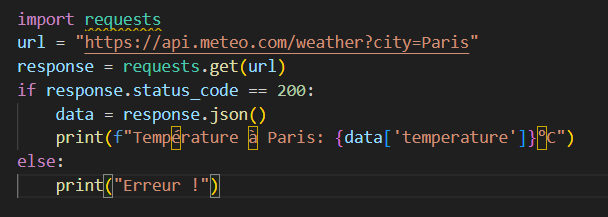
\includegraphics[width=0.87\textwidth]{exemple.png}
		\end{center}
	\end{exampleblock}
	
\end{frame}

% Section 7 : Bonnes pratiques
\section{Bonnes pratiques}
\begin{frame}{Bonnes pratiques}
	\begin{itemize}
		\item \textbf{Documentation} : Consultez toujours la documentation officielle de l'API pour comprendre son fonctionnement.
		\item \textbf{Gestion des erreurs} : Anticipez les erreurs (exemple : requêtes échouées ou serveur indisponible).
		\item \textbf{Sécurité} : Utilisez HTTPS, des tokens d'authentification et vérifiez les permissions.
	\end{itemize}
\end{frame}


% Section 8 : Outils pour tester les API
\section{Outils pour tester les API}
\begin{frame}{Outils pour tester les API}
	\begin{itemize}
		\item \textbf{Postman} : Interface graphique pour tester, documenter et automatiser des requêtes API.
		\item \textbf{cURL} : Outil en ligne de commande pour envoyer des requêtes HTTP.
		\item \textbf{Insomnia} : Alternative à Postman, simple et efficace pour tester des APIs.
	\end{itemize}
\end{frame}


% Section 9 : Importance des API
\section{Pourquoi c'est important ?}
\begin{frame}{Pourquoi c'est important ?}
	\begin{itemize}
		\item Les API sont omniprésentes : réseaux sociaux, applications mobiles, IoT.
		\item Elles permettent de développer des solutions interconnectées et évolutives.
		\item Gain de temps et de ressources grâce à la réutilisation des services existants.
	\end{itemize}
\end{frame}




\end{document}
